%%%%%%%%%%%%%%%%%%%%%%%%%%%%%%%%%%%%%%%%%%%%%%%%%%
%%%%		~~~~ Method ~~~~
%%%%%%%%%%%%%%%%%%%%%%%%%%%%%%%%%%%%%%%%%%%%%%%%%%


\chapter{Open string spectrum}
\label{chap:spectrum}
\pagestyle{fancy}

In this chapter we will describe the spectrum of D-brane systems in the context of type IIB String Theory. We start by discussing single brane spectrums, and then move on to general brane configurations, to conclude with the main example of this thesis, the D1/D5 brane system.

\section{Dp-Dp spectrum}

%Discuss the spectrum of a single Dp-brane. Start with D9 SYM and dimensionally reduce.

Consider a single D9-brane. This equates to considering Neumann boundary conditions in all directions of a string. The NS vacuum is a scalar $\ket{0}$, while the R sector is a spinor $\ket{a}$, given by $SO(2)$ eigenvalues $s_0, s_1, s_2, s_3, s_4$. The massless spectrum can be found from the mass formula $\alpha ' M^2 = N + 1/2$. This leads to the modes $b_{-1/2}^\mu \ket{0}$ and $\ket{a}$.

The representation theory of the massless spectrum turns out to be straight forward. There is a vector and a fermion in D = 10, composed by $b_{-1/2}^\mu \ket{0}$ and $\ket{a}$ respectively.

To obtain the spectrum of an arbitrary Dp-brane we can perform dimensional reduction over the D9 spectrum we already constructed. By dimensional reduction we mean splitting the D9 symmetry group $SO(1,9)$ into the transverse and world-volume symmetry groups of the lower dimensional Dp-brane, namely, $SO(1,p) \times SO(9-p)$. 

Starting with a vector in the $\mathbf{10}$ of $SO(1,9)$, it decomposes into a $(\mathbf{p},\mathbf{1}) \oplus (\mathbf{1}, \mathbf{9-p})$ of $SO(1,p)\times SO(9-p)$. The original R vacua was a Majorana-Weyl spinor of $SO(1,9)$, and depending on $p$ it will decompose into the corresponding irreducible spinors of $SO(1,p)\times SO(9-p)$. The dimensional reduction of spinors is discussed in detail in \ref{ap:spinors}.

This is already the full spectrum of a single Dp-brane. Extending it to a stack of $Q_p$ Dp-branes adds a Chan-Paton factor to both string ends, which labels the adjoint representation of $U(Q_p)$. 

We can count on-shell degrees of freedom to make sure the spectrum is supersymmetric. For a explicit example, we can consider a single D5-brane. By on-shell we refer to adopting light-cone gauge, meaning that $SO(1,5) \rightarrow SO(4)$, effectively identifying 2 degrees of freedom for the vector, and specifying a $s_0$ eigenvalue for the spinor.

\begin{align*}
    (\mathbf{6},\mathbf{1}) \rightarrow (\mathbf{4},\mathbf{1}\\
    (\mathbf{1},\mathbf{4}) \rightarrow (\mathbf{1}, \mathbf{4})\\
    (\mathbf{4}_s,\mathbf{2}_s) \rightarrow (\mathbf{2}_s,\mathbf{2}_s) \\
    (\mathbf{4}_c,\mathbf{2}_c) \rightarrow (\mathbf{2}_c,\mathbf{2}_c) \\
\end{align*}

Now if we count degrees of freedom in the right side, we find that there are 8 matching bosonic and fermionic degrees of freedom, meaning that there can be 8 on-shell supercharges in the theory. A general discussion can be made for any $p$ to find the same 8 possible on-shell supercharges. 

\section{Dp-Dp' spectrum}

%Start by finding the vacuum. See how it is like a full R vacuum split as a tensor product

Now consider two D branes of arbitrary dimensions $p$, $p'$. In general, some of the directions will have the same boundary conditions, i.e. DD or NN, while some will have mixed boundary conditions, i.e. DN or ND. This is illustrated in Figure \ref{fig:brane-schematic}.


\begin{figure}[htbp]
    \centering
    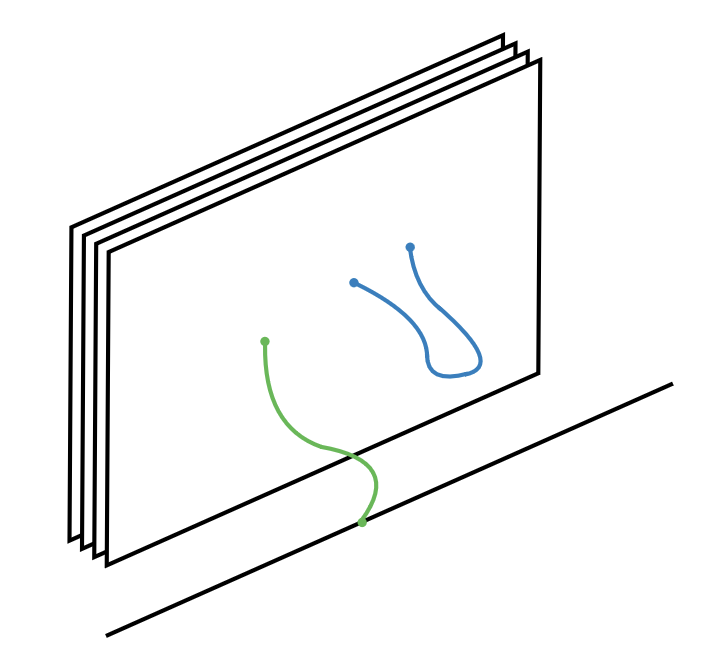
\includegraphics[width=0.5\textwidth]{IMAGES/brane-strings.png}
    \caption{Schematic representation of a stack of Dp branes and a single Dp' brane with strings attached. The blue string will have the same boundary conditions in all directions while the green string will have mixed conditions in some. Figure taken from \cite{Stemerdink:2022hnf}.}
    \label{fig:brane-schematic}
\end{figure}

As we did for the single D brane, the boundary conditions will lead to a relation between left and right moving modes. 

\begin{align}
    \text { NN: } X^\mu(z, \bar{z}) & =x^\mu-i \alpha^{\prime} p^\mu \ln (z \bar{z})+i \sqrt{\frac{\alpha^{\prime}}{2}} \sum_{m \neq 0} \frac{a_m^\mu}{m}\left(z^{-m}+\bar{z}^{-m}\right) \\
    \text { DN, ND: } X^\mu(z, \bar{z}) & =i \sqrt{\frac{\alpha^{\prime}}{2}} \sum_{r \in \mathbb{Z}+1 / 2} \frac{a_r^\mu}{r}\left(z^{-r} \pm \bar{z}^{-r}\right) \\
    \text { DD: } \quad X^\mu(z, \bar{z}) & =-i \frac{\delta X^\mu}{2 \pi} \ln (z / \bar{z})+i \sqrt{\frac{\alpha^{\prime}}{2}} \sum_{m \neq 0} \frac{a_m^\mu}{m}\left(z^{-m}-\bar{z}^{-m}\right)
\end{align}

Notice that the moding for the ND/DN directions gets shifted by $1/2$ to accomodate the mixed boundary conditions. This property is also apparent on the fermions 

Once again, we aim to calculate the massless spectrum. Thus, we want to find the zero point energy in both the R and the NS sector. As per usual, the R vacuum is massless, while the zero point energy for the NS sector is,

\begin{equation}
    \label{eq:zero-point-mixed}
    -\frac{1}{2} + \frac{\nu}{8}
\end{equation}

\section{D1/D5 spectrum}

The D1/D5 brane system will be the main example treated in this thesis. It deserves a propper introduction, so first of all let's define it in detail. Consider a stack of $Q_5$ D5 branes covering the 5, 6, 7, 8, 9 directions. Next, consider a stack of $Q_1$ D1 branes laying inside the D5 stack in the 5 direction. Table \ref{table:D1/D5} gives a summary of what was described.

\begin{table}[h]
    \centering
    \begin{tabular}{|l|l|l|l|l|l|l|l|l|l|l|}
    \hline
       & 0 & 1 & 2 & 3 & 4 & 5 & 6 & 7 & 8 & 9 \\ \hline
    D1 & - & . & . & . & . & - & . & . & . & . \\ \hline
    D5 & - & . & . & . & . & - & - & - & - & - \\ \hline
\end{tabular}
\caption{Schematic representation of the D1/D5 system.}
\label{table:D1/D5}
\end{table}

As we can see, the number of mixed directions is $\nu = 4$, so from equation \ref{eq:zero-point-mixed}, the zero point energy of the NS sector of 1-5 and 5-1 string vanishes. Then, the massless spectrum of excitations of these strings will be both the R vacuum and the NS vacuum. Take for instance a 1-5 string, meaning that the endpoint at $\sigma = 0$ lays in the D1 brane, while the one at $\sigma = \pi$ lays in the D5 brane. The bassless modes will be generated by,

\begin{align}
    \label{eq:zero-modes-d1d5}
    \text{NS: } &b_0^i, \quad i=6,7,8,9\\
    \text{R: }  &b_0^M, \quad M = 0,1,2,3,4,5
\end{align}

Both of these sectors generate Clifford algebras separately of the respective subgroups of $SO(1,9)$. At first glance, we could think the important subgroup is $SO(1,5) \times SO(4) \subset SO(1,9) $, but as it was mentionied previously, we want to focus on the theory on the intersection world-volume, so we want to look at the subgroup $SO(1,1) \times SO(4)_I \times SO(4)_E \subset SO(1,9)$, where the subindices indicate the directions 1, 2, 3, 4 for I and 6, 7, 8, 9 for E.

According to this splitting, the Clifford algebras of Equations \ref{eq:zero-modes-d1d5} generate spinors of $SO(1,5)$ and $SO(4)_I$ respectively. The $SO(1,5)$ spinor then splits into various $SO(1,1) \times SO(4)_E$ spinors.

Let's consider the R vacuum given by the $SO(1,5)$ spinor $\ket{s_0, s_1, s_2}$. The GSO projection picks one $SO(1,5)$ chirality, and in this case we decide it picks the $\mathbf{4}_s$.

We pick a basis where the first eigenvalue $s_0$ is associated to the 0, 5 directions, while the other are associated to the 1, 2, 3, 4 directions. This is convenient because the spinor splits as $\ket{s_0} \otimes \ket{s_1, s_2}$ under $SO(1,9) \rightarrow SO(1,1) \times SO(4)_E$. Now, counting chiralities in $SO(1,1)$ and $SO(4)_E$ we can see that this spinor fills the representations $(\mathbf{1}_s, \mathbf{2}_s) \oplus (\mathbf{1}_c, \mathbf{2}_c)$.

A similar, albeit easier calculation, shows that the NS vacuum is characterized by a $SO(4)_I$ spinor in the $\mathbf{2}_s$.

At last, the spectrum of the 1-5 string can be obtained by noticing that in the NS sector all states are $SO(4)_I$ singlets, while in the R sector they are $SO(1,1) \times SO(4)_E$ singlets, i.e,

\begin{align}
    \text{NS: } (\mathbf{1}_s, \mathbf{2}_s, \mathbf{1}) \oplus (\mathbf{1}_c, \mathbf{2}_c, \mathbf{1}) \\
    \text{R: } (\mathbf{1}, \mathbf{1}, \mathbf{2}_s)
\end{align}

Note that the 5-1 strings will produce the same zero modes, so that the vacuum will be identical.

The only missing piece at this point it the 1-1 and 5-5 massless spectrums. We already know that these come from the dimensional reduction of the $\mathbf{10}$ and the $\mathbf{16}_s$ of $SO(1,9)$. It is straight forward to see that the vector decomposes as $(\mathbf{2},\mathbf{1},\mathbf{1})\oplus(\mathbf{1},\mathbf{4},\mathbf{1}) \oplus(\mathbf{1},\mathbf{1},\mathbf{4})$. The procedure to decompose the spinor is very similar to what we did with the $\mathbf{4}_s$ of $SO(1,5)$ previously. Now we need to split the $\mathbf{16}_s$ via the eigenvalues $s_0$ in $SO(1,1)$, $s_1$, $s_2$ in $SO(4)_E$ and $s_3$, $s_4$ in $SO(4)_I$. Again, counting chiralities we end up with,

\begin{equation*}
    \mathbf{16}_s \rightarrow (\mathbf{1}_s, \mathbf{2}_s, \mathbf{2}_s) \oplus (\mathbf{1}_s, \mathbf{2}_c, \mathbf{2}_c) \oplus (\mathbf{1}_c, \mathbf{2}_c, \mathbf{2}_s) \oplus (\mathbf{1}_c, \mathbf{2}_s, \mathbf{2}_c)
\end{equation*}

